\documentclass[conference]{IEEEtran}
% \IEEEoverridecommandlockouts
% The preceding line is only needed to identify funding in the first footnote. If that is unneeded, please comment it out.
\usepackage{cite}
\usepackage{amsmath,amssymb,amsfonts}
\usepackage{algorithmic}
\usepackage{hyperref}
\usepackage{graphicx}
\usepackage{textcomp}
\usepackage{xcolor}
\def\BibTeX{{\rm B\kern-.05em{\sc i\kern-.025em b}\kern-.08em
    T\kern-.1667em\lower.7ex\hbox{E}\kern-.125emX}}
\begin{document}

\title{Computer Technology Project I\\}

\author{\IEEEauthorblockN{Simon Nyman}
\IEEEauthorblockA{\textit{Dept. of Electrical and Computer Engineering} \\
\textit{Aarhus University}\\
Studentnumber: 202305077\\}
\and
\IEEEauthorblockN{Jakob Palm}
\IEEEauthorblockA{\textit{Dept. of Electrical and Computer Engineering} \\
\textit{Aarhus University}\\
Studentnumber: 202307244\\}
}

\maketitle

\begin{abstract}
\end{abstract}

\section{Introduction}
The goal for this project was to design a down-scaled version of a Search And Rescue (SAR) robot, used to rescue victims in the aftermaths of natural disasters.
The robot will imitate a real world scenario by, autonomously navigating an obstacle course and distinguishing between different color markings, representing potential victims. To achieved this we use the TurtleBot3 Burger Robot equipped with different sensors.
All the software will be implmented in python using the Robot Operating Software framework (ROS). For the sensors we will be using a LiDAR sensor capable of measuring distances in a 360 degree view, and an RGB-sensor which differentiates between red, green and blue colors. 
The performance will be assessed based on three factors: Average speed, number of collisions and "victims" found.

\section{Specifications}
Our Search and Rescue implementation used a turtlebot3 robot, specifically the burger configuration with dimensions 138mm x 178mm x 192mm (L $\times$ W $\times$ H)\cite{b1}.
On the turtlebot3, a Raspberry Pi 3 model B+ and an Arduino are connected in order to process the incoming external signals from the various sensors.
Furthermore, the robot has two motors attached, one for each wheel. From the specification it is evident that the robot has a maximal linear velocity of 0.22 m/s
and a maximum rotational velocity of 2.84 rad/s. In order keep the robot as agile as possible with no wires attached, we used an 800 mA Li-Po battery and established a wireless connection, which will be specified further in a following section.
The specific RGB used is an ISL29125 low power, high sensitivity red, green and blue light sensor with SMBus compatibility\cite{b2}.
The LiDAR used is the LDS-01 version with a range of 120 mm to 3500 mm, capable of doing full 360 degree scans. \cite{b3}

\subsection{Software Setup}

\subsubsection{Network Configuration}
As mentioned, we wanted the robot to be able to move as freely as possible, meaning that connecting it to our machine via an ethernet cable was not the way to go.
Therefore, we established a wireless connection to the robot by changing the network configuration on the sd card, making it automatically connect to the IP-address of our machine.
This allowed for easy connection to the robot once a mobile hotspot was opened, as the robot was automatically allocated an IP-address.
With this configured, the robot would subscribe to our machine on which the required ROS environments (these will be specified in the nect section) would publish actuation data to the motors of the robot, enabling wireless navigation.

\subsubsection{ROS}

The ROS operating system proved to be very useful in regards to this project, as it provided a very useful framework for our specific problem.
The three main parts used were topics, messages, and nodes (rostopic, rosmsg, rosnode). These are all integral parts of the ROS framework, as each provides a unique functionality in abstracting the navigation.
Nodes are responsible for performing computations and communicate internally through topics, while messages are used for communicating with the external sensors.

In our case, we had three nodes running. One running roscore, which encapsulates the entire framwork, allowing the other nodes to run in the ROS environment.
The second node ran the basic functionality of the robot, such as managing the incoming sensor data and sending signals to the motors.
The third node was running the navigation code that we wrote. These communicated by the subsribe/publish model to send data back and forth, in order to control the navigation of the robot.
The nodes also contain debug information and allowed us to log the information we required for optimizing and reason about the relevant aspects of the code as we were testing it.


\section{Methodology and Design}
Throughout the project we have been using the trial and error approach, which allowed for an efficient overall workflow. 
This approach works well, when having to build and optimize code for hardware, as we would need to see if and how the code is working and reasoning about it on an abstract level would only get us so far.
Furthermore, this approach works in great synergy with the See-Think-Act Cycle we use for the robot, see \href{sec:STAC}{Fig. 1}.
We are able to edit the "see", "think" and "act" parts individually and get instant feedback by testing, as this approach to navigation is very straight forward to reason about, simplifying both the building and optimization processes.
\begin{figure}[htbp]
    \centerline{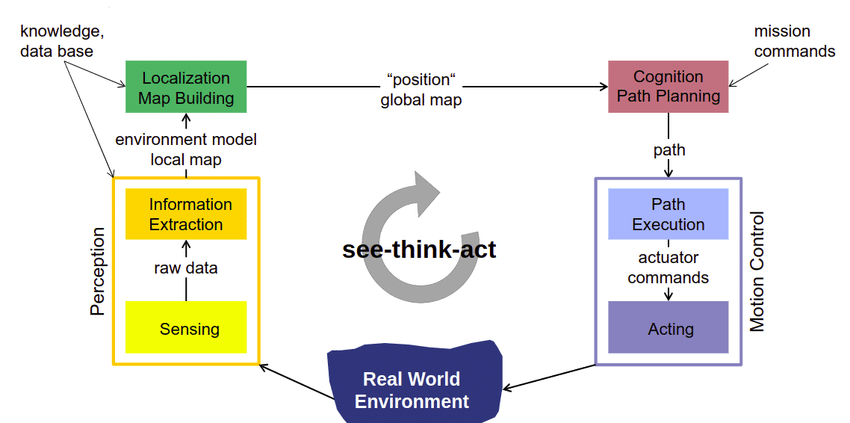
\includegraphics[width=1.0\columnwidth]{STAC.png}}
    \caption{Robots See-Think-Act Cycle.}
    \label{sec:STAC}
    \end{figure}

\subsection{LiDAR}
The use of LiDAR readings is an integral part of the design, as the entire navigation logic depends upon these.
In our implementation, it had two use cases, one being the ability to read in which direction the nearest obstacle was present, if any, and the second being the ability to read the specific distance to said obstacle, which would determine what to do next.
As the LiDAR provides a 360 degree scan, we first had to figure out which angles to use and how these were organized within the LiDAR.
By firstly playing around with the angles, we figured out that they were organized in a way such that 0$^\circ$ was at the back of the robot, and then continued clockwise around the robot.
This meant that the front 180$^\circ$ were located in the interval $[90:270]$. How this was used in our final implementation will be elaborated on in the \textit{Navigation} section.
During initial testing of the LiDAR, we encountered a problem, as some angles seemed to not be working properly and would either give readings very close to 0, which resulted in the robot refusing to move, or infinitely large readings.
To fix this, we wrote a loop within the LiDAR scan function, which would iterate through the values in the angles being read and, if any angles were suffering from either of these problems, would fix them, as seen in \href{sec:lidar}{Fig. 2}.
If the value was infinitely large, it would set it to the max value of the LiDAR, which, as previously mentioned, is 3.5 meters.
In the case that an angle gave readings very close to 0, it would set this to 1 meter as this would have no impact on the other readings.
We had a third case, which checked whether the reading was indeed a number as it should, and would otherwise set it to 0 in which case it would be ignored as described.
With this configured, we additionally addded a few centimeters to each reading due to the innate imprecision of the LiDAR, which will be apparent later on.
\begin{figure}[htbp]
    \centerline{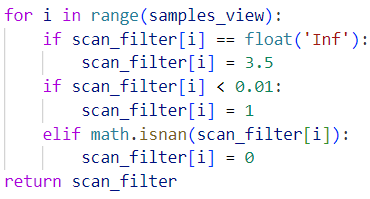
\includegraphics[width=0.6\columnwidth\hspace{-1.3cm}]{LiDARhvid.png}}
    \caption{Ignoring the dead LiDAR angles.}
    \label{sec:lidar}
    \end{figure}


\subsection{Navigation}
\begin{figure}[htbp]
    \centerline{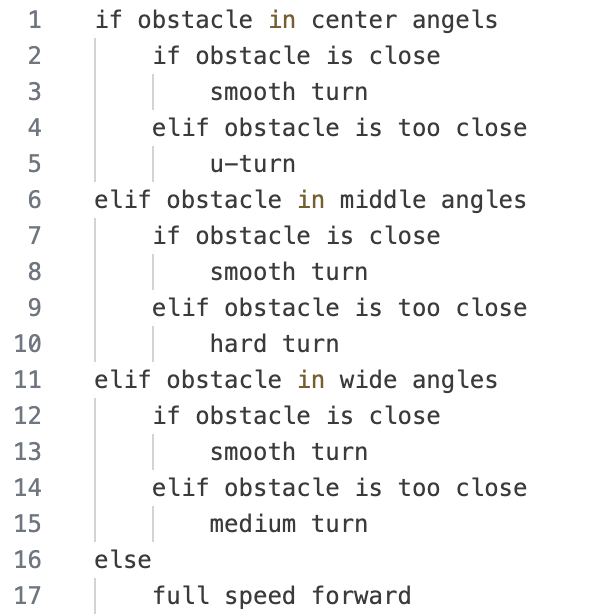
\includegraphics[width=0.6\columnwidth\hspace{-1.3cm}]{Pseudo.png}}
    \caption{.}
    \label{sec:pseudo}
    \end{figure}
\begin{figure}[htbp]
    \centerline{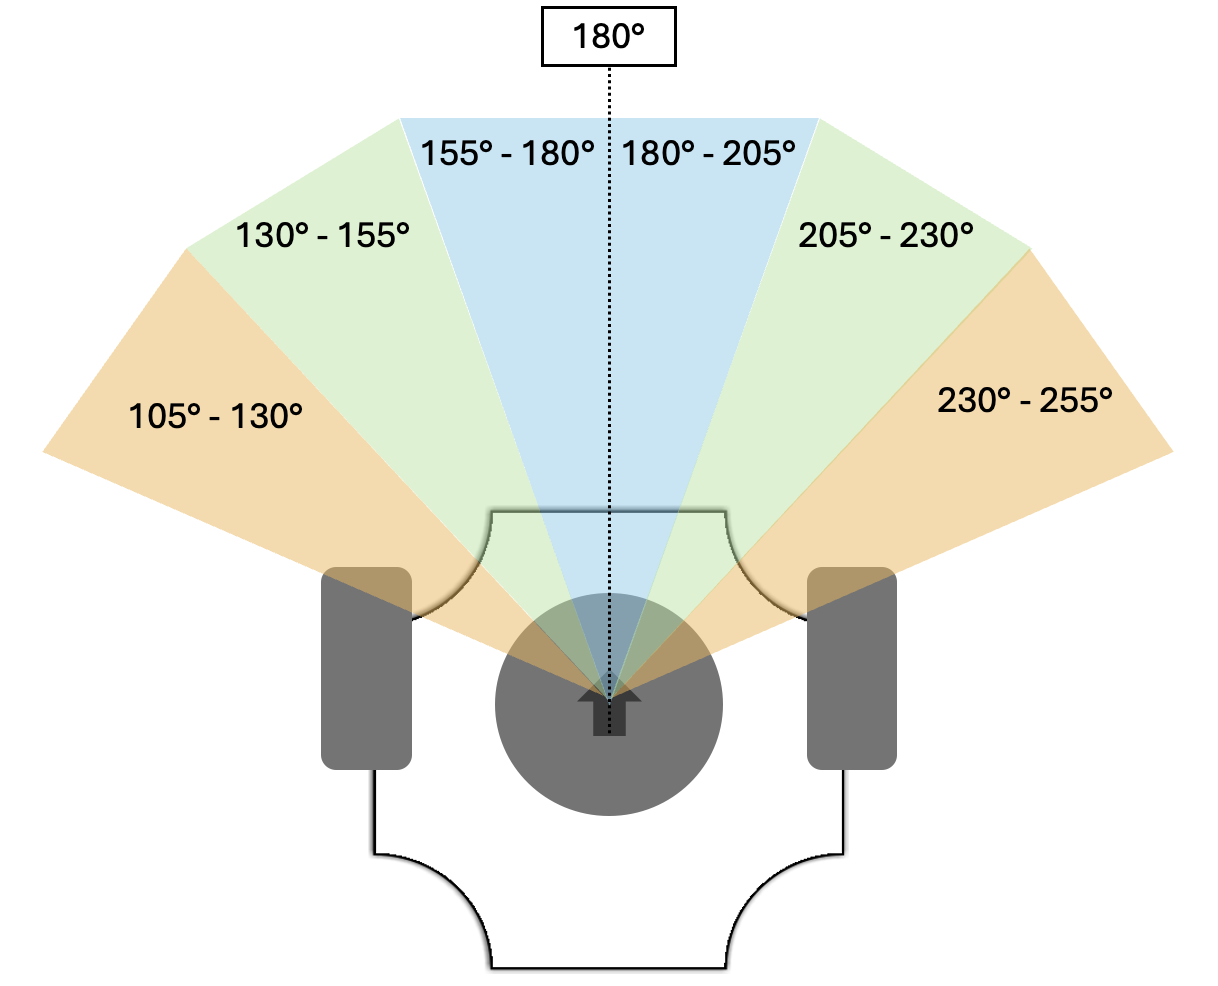
\includegraphics[width=0.9\columnwidth]{LiDAR Angels.png}}
    \caption{.}
    \label{sec:angles}
    \end{figure}
\begin{figure}[htbp]
    \centerline{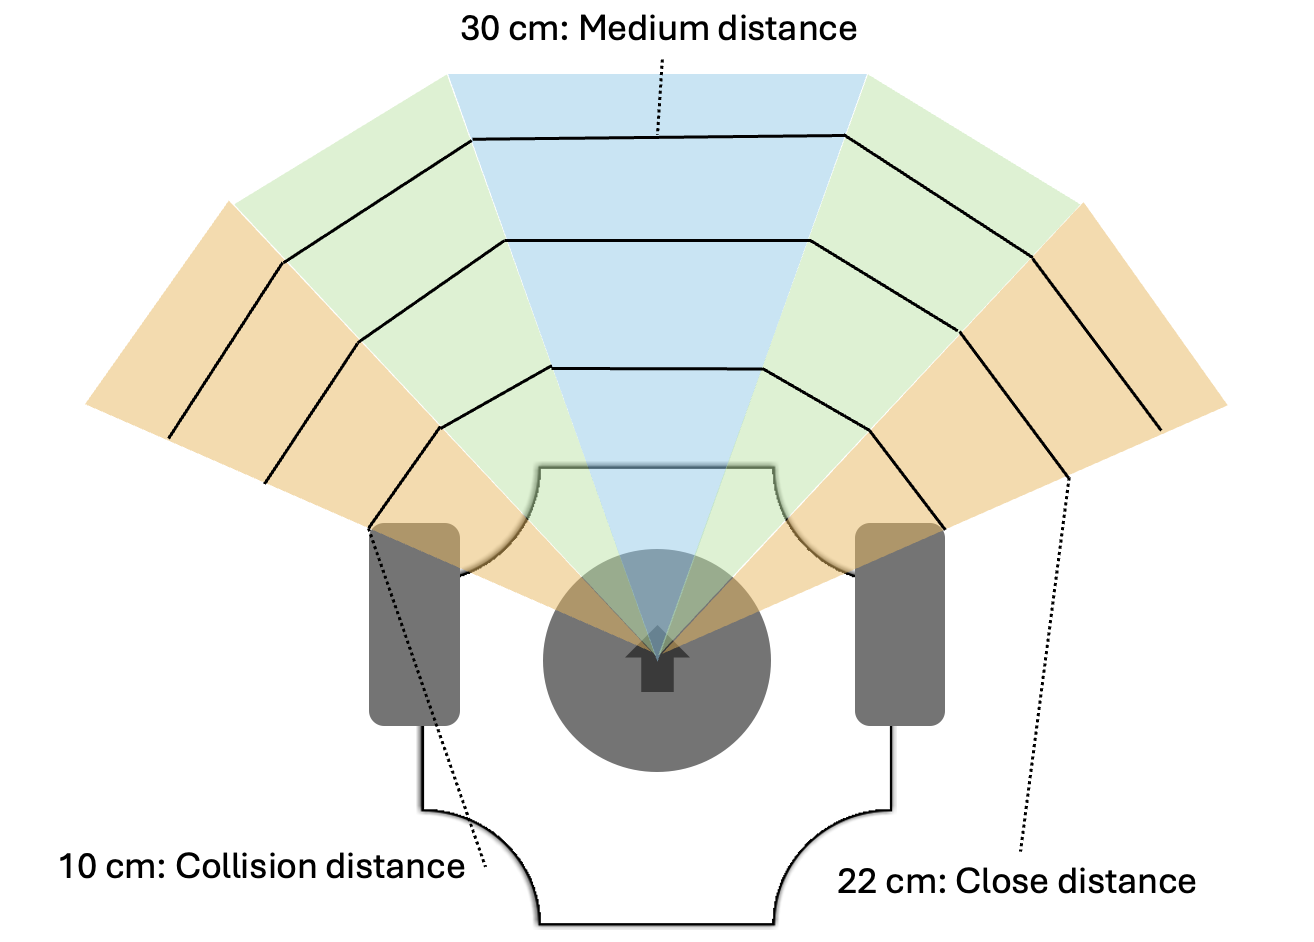
\includegraphics[width=0.9\columnwidth]{LiDAR Distances.png}}
    \caption{.}
    \label{sec:distances}
    \end{figure}
\begin{figure}[htbp]
    \centerline{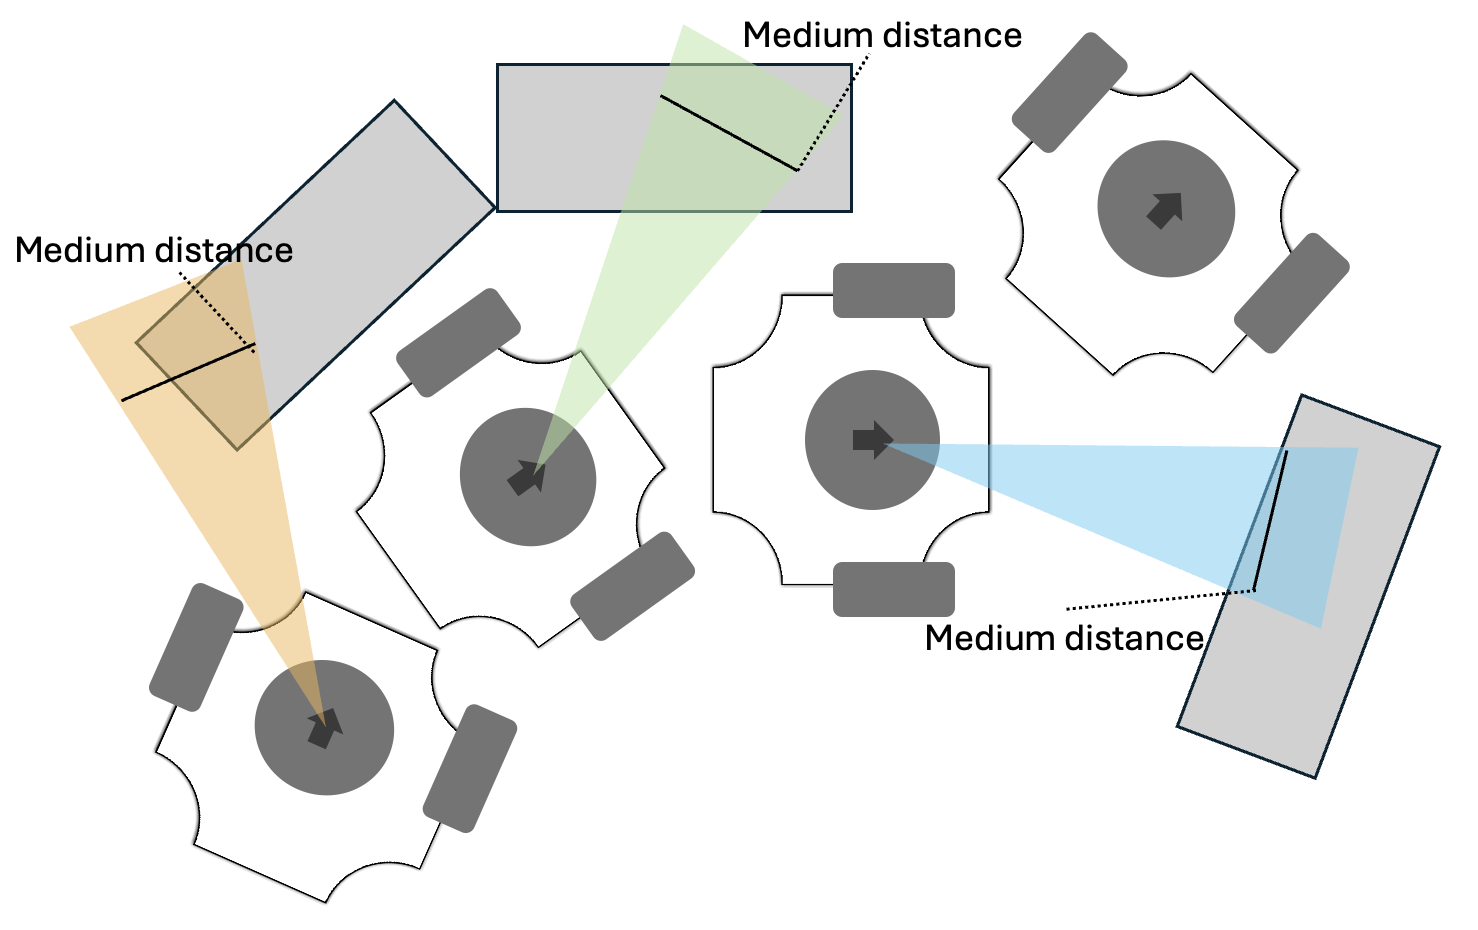
\includegraphics[width=0.9\columnwidth]{Medium Distance Aviodance.png}}
    \caption{.}
    \label{sec:medium aviodance}
    \end{figure}
\begin{figure}[htbp]
    \centerline{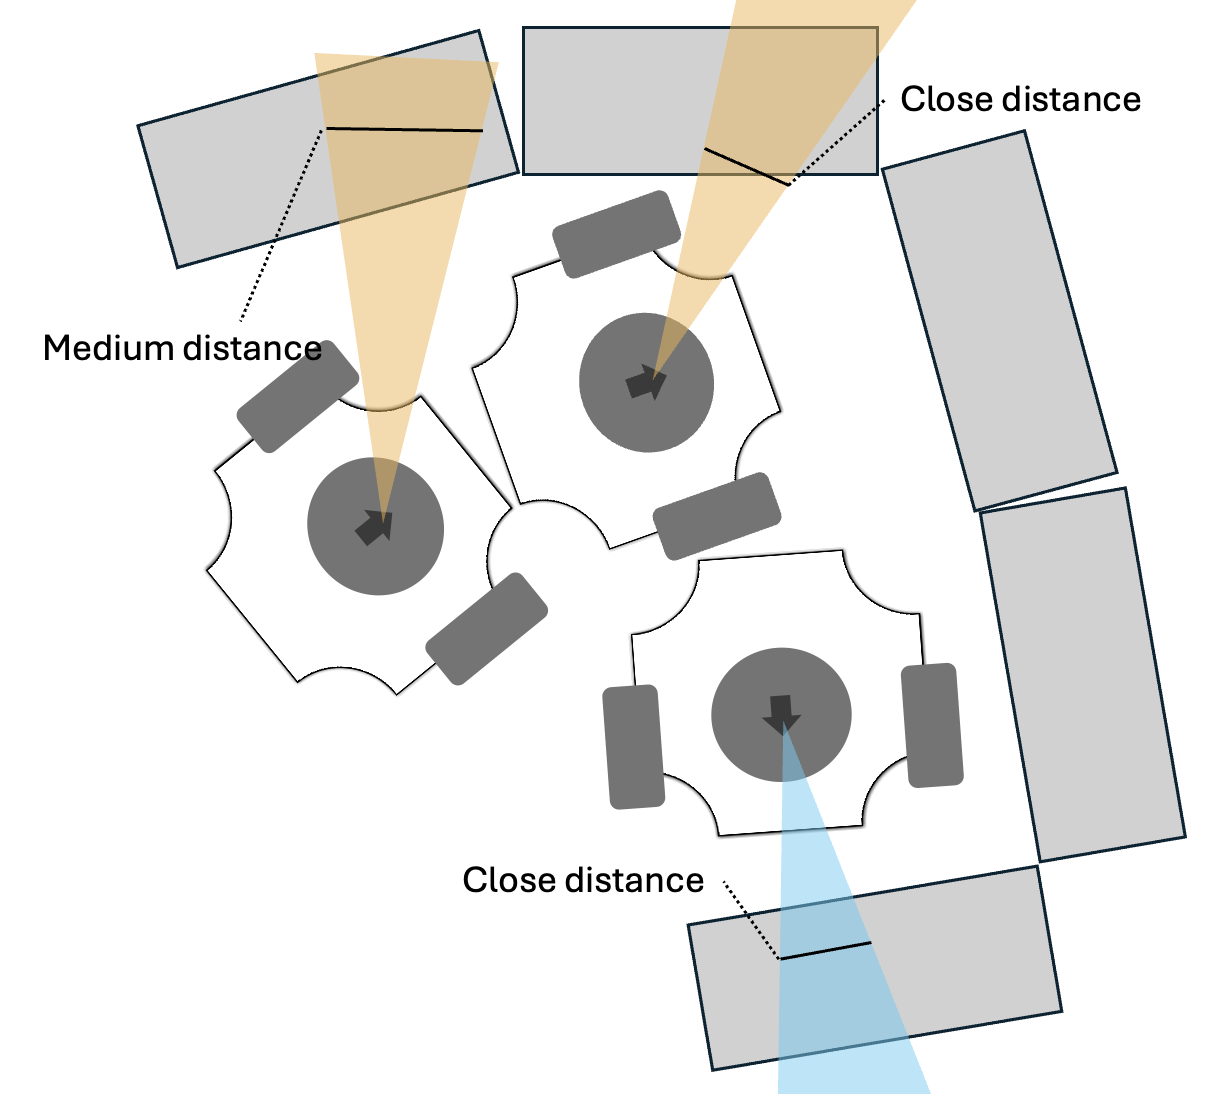
\includegraphics[width=0.9\columnwidth]{Close Distance Avoidance.png}}
    \caption{.}
    \label{sec:close aviodance}
    \end{figure}
implementation
\subsection{RGB}
implementation
\subsection{LED}
implementation
\section{Experimentation and Testing}

\section{Conclusion}

\section{Discussion}

\section{Personal Contributions}

\subsection{Simon Nyman}
Contributed nothing, a waste of space

\subsection{Jakob Palm}
Actually did the entire thing.

\begin{thebibliography}{00}
\bibitem{b1} 'Turtlebot3 features', accessed 15 May 2024, available at: https://emanual.robotis.com/docs/en/platform/turtlebot3/features/
\bibitem{b2} 'Renesas RGB-sensor ISL29125 datasheet', accessed 15 May 2024, available at: https://www.alldatasheet.com/datasheet-pdf/pdf/1045936/RENESAS/ISL29125.html
\bibitem{b3} 'LDS-01 overview', accessed 15 May 2024, available at: https://www.robot-advance.com/EN/art-360-laser-distance-sensor-lds-01-2352.htm
\end{thebibliography}

\end{document}
